\documentclass[10pt]{beamer}

\usetheme{metropolis}
\usepackage{appendixnumberbeamer}
\usepackage{hyperref}
\usepackage{graphicx}
\usepackage{booktabs}
\usepackage[scale=2]{ccicons}
\usepackage{subfig}
\usepackage{pifont}
\newcommand{\cmark}{\ding{51}}%
\newcommand{\xmark}{\ding{55}}%

\usepackage{pgfplots}
\usepackage{threeparttable}
\usepgfplotslibrary{dateplot}

\usepackage{natbib}
\usepackage{colortbl}
\usepackage{lmodern}
\usepackage{multirow}
\usepackage{tikz}

\newcommand{\beqns}{ \begin{eqnarray*} }
\newcommand{\eeqns}{ \end{eqnarray*} }

\newcommand{\bitem}{\begin{itemize}}
\newcommand{\eitem}{\end{itemize}}
\newcommand{\benu}{\begin{enumerate}}
\newcommand{\eenu}{\end{enumerate}}



\usepackage{xspace}
\newcommand{\themename}{\textbf{\textsc{metropolis}}\xspace}

%this data comes from https://data.worldbank.org/indicator/SL.UEM.1524.ZS?locations=ID
%They are ILO estimates. They have nothing to do with the Indonesian statistics.

\newcommand{\idnur}{16.1}
\newcommand{\seaur}{10.4}


\title{Local labor markets, population density and the gender gap}
\date{\today}
\author{C\'esar Garro-Mar\'in}
\institute{Boston University}
\begin{document}

\maketitle

\section{Introduction}
\begin{frame}{Summary} 
	In the next slides I document three main facts about the \alert{\textbf{gender gap}} in the US for the period of 1970 and 2020:
	\benu
		\item There is a large dispersion in the \textbf{\alert{level}} of the gender wage gap across labor markets in the US. The dispersion persists despite the general decrease in the level of the gap since 1970.
		\item There are differences in the \textbf{\alert{change}} of the gender wage gap. The largest reductions happened in densest labor markets.
		\item The relationship between the \textbf{\alert{level}} of gender wage gap and population density has inverted over the period. Today, the densest labor markets have a lower gender wage gap.
	\eenu
\end{frame}

\section{Data}
\begin{frame}{Data}
	\textbf{\alert{Source:}} IPUMS data for:
		\bitem 
		\item 1950-2000 Decennial censuses.
		\item 5-year ACS for the years 2011 and 2018. For ease of presentation I label these datasets as 2010 and 2020 respectively.
	\eitem
	\textbf{\alert{Sample}} includes all full-time year-round workers whom:
	\bitem
		\item Aged 18-64.
		\item Not attending school.
		\item Not living in group quarters.
		\item For all graphs I limit the sample to people living in CZ with a population density of at least 1 person per-square kilometer in 1950.
	\eitem
\end{frame}
\section{Empirical facts}

\begin{frame}{Fact 1: there is substantial variation in the gender gap across CZ} 
\begin{figure}[!h]
\centering
\caption{The gender gap in the US in 2020}
\label{fig:gap_map2020}
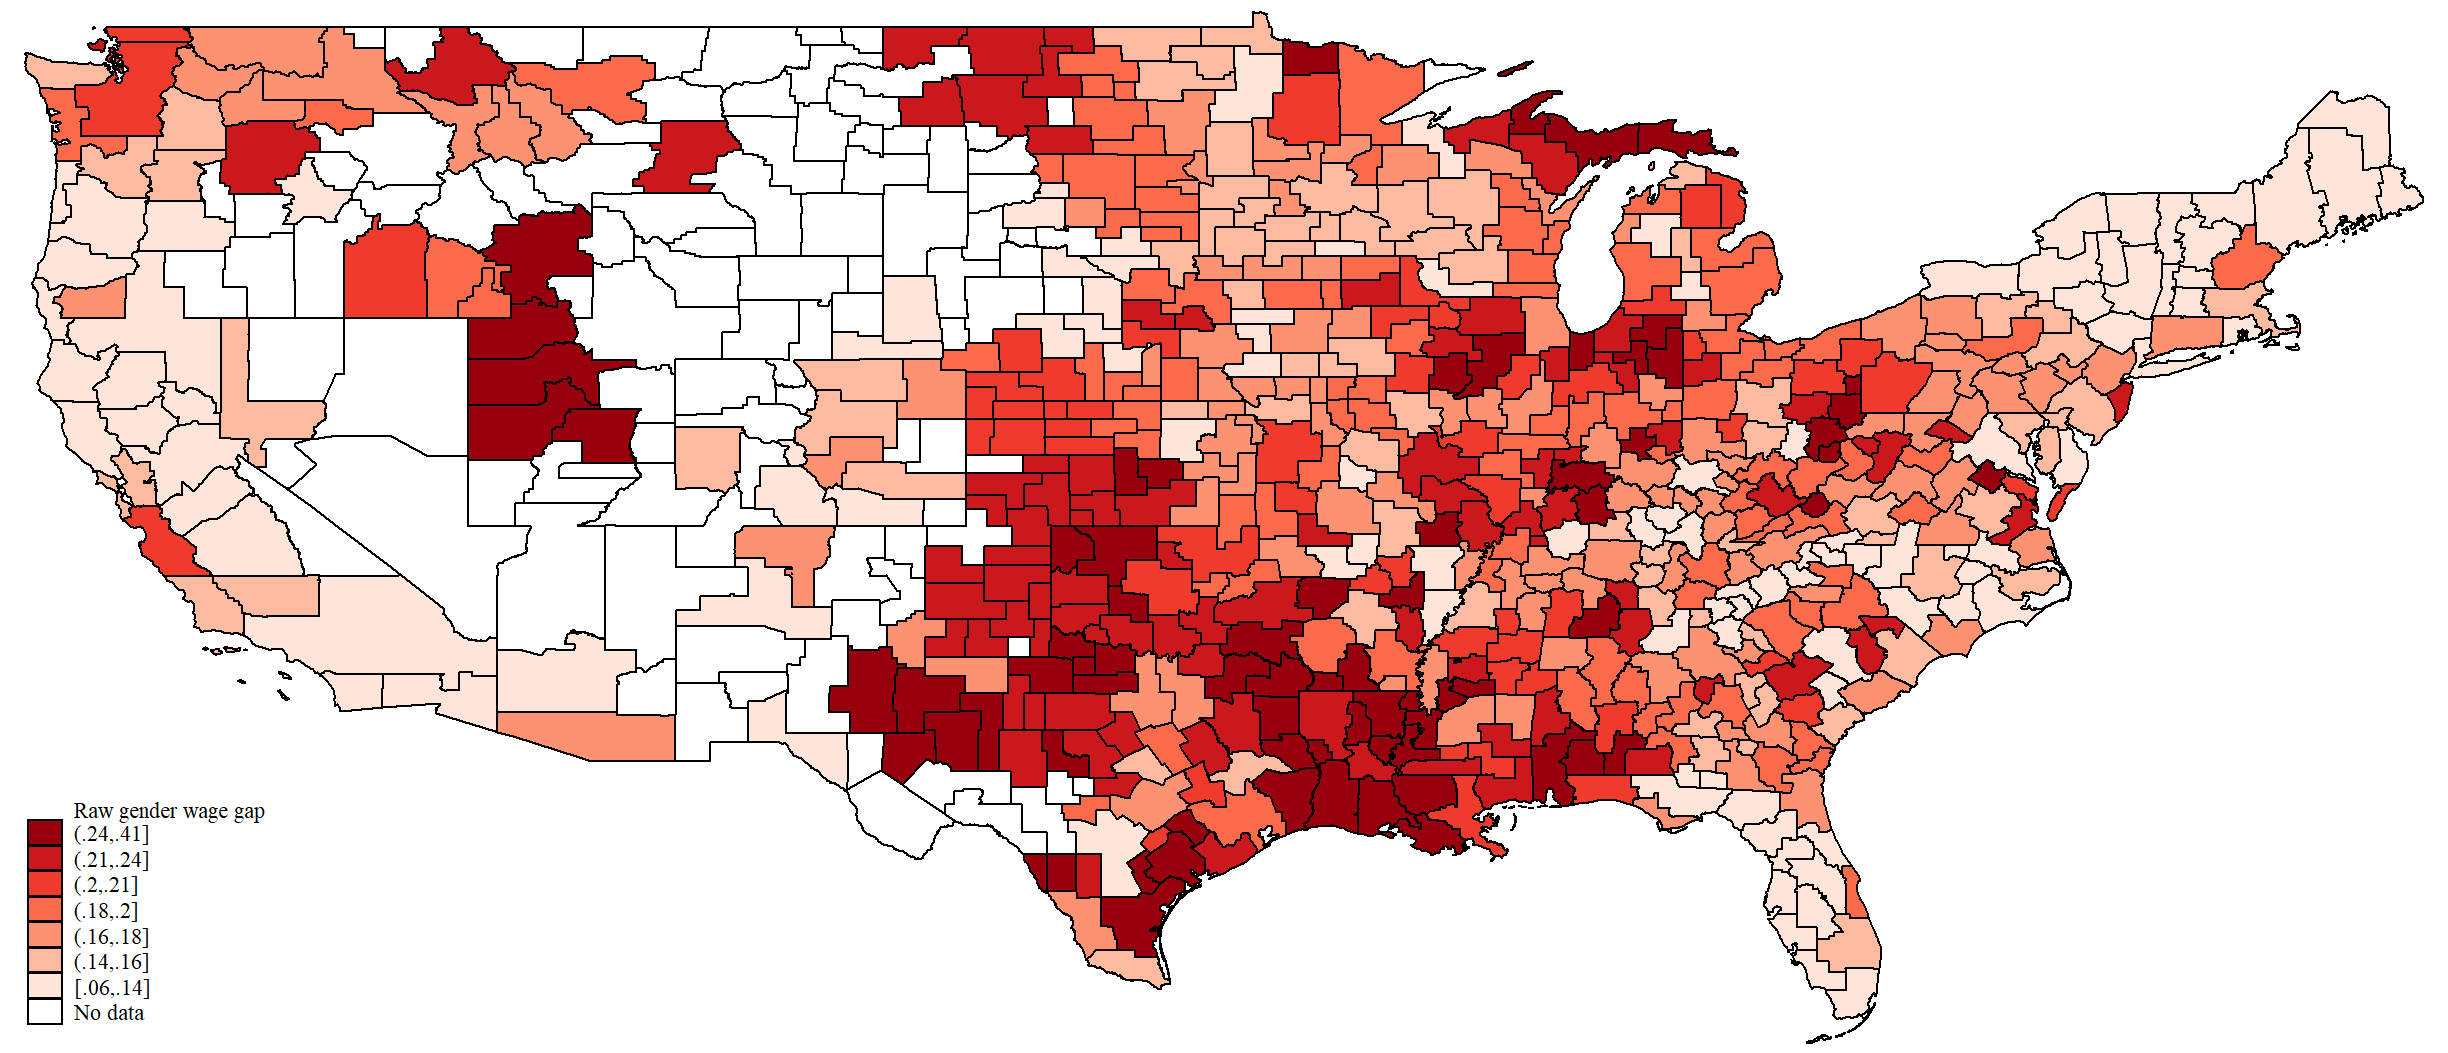
\includegraphics[width=1\textwidth]{../2_analysis/output/figures/raw_wage_map2020_full_time}
\par \begin{minipage}[h]{\textwidth}{\tiny\textbf{Note:} darker colors denote higher relative wages for men. Figure restricts to czones with population densities above 1 person per km$^2$ and full-time year-round workers.}\end{minipage}
\end{figure}

\end{frame}
\begin{frame}{Fact 1: Cross-CZ variation persists despite general decline at the national level}
	\begin{figure}[!h]
\centering
\caption{Evolution of raw gender gap across CZ}
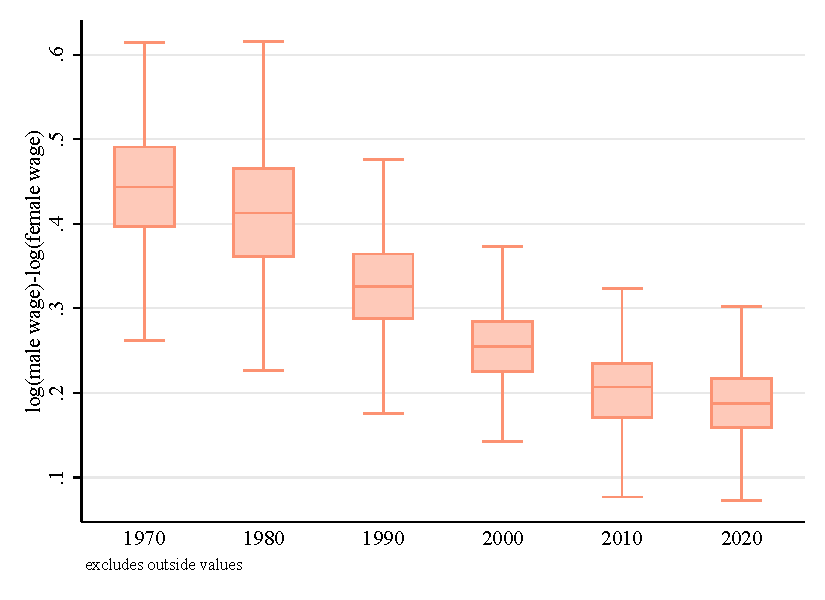
\includegraphics[width=.6\textwidth]{../2_analysis/output/figures/cz_gap_dispersion_full_time}
\par \begin{minipage}[h]{\textwidth}{\scriptsize\textbf{Note:} figure restricts to CZ with more than people per km$^2$ and full-time year-round workers..}\end{minipage}
\end{figure}

\end{frame}
\begin{frame}{Cross-CZ gender gap differences are persistent}
	\textbf{\alert{Regression specification:}} $w^{men}_{rt}-w^{women}_{rt}=\alpha_{rt}+\beta_{t}(w^{men}_{rt-j}-w^{women}_{rt-j})$
	\begin{figure}[!h]
\centering
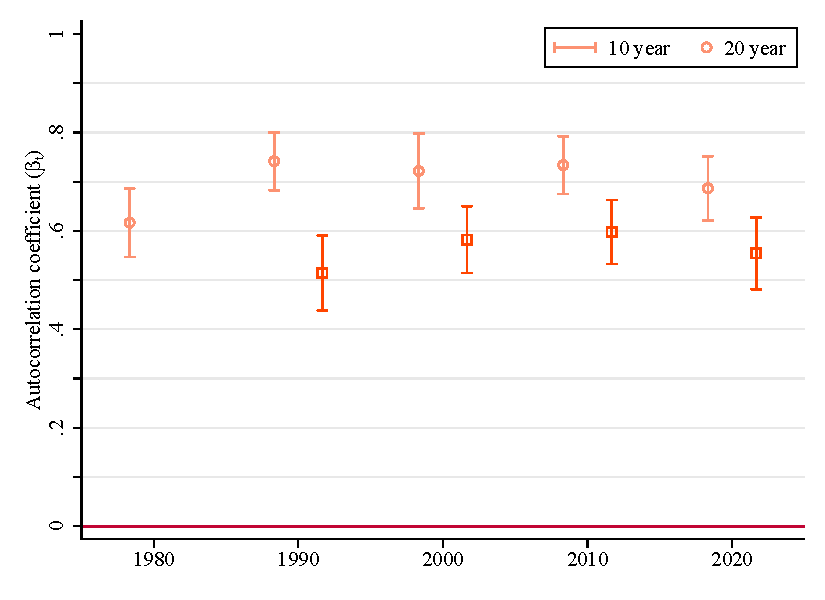
\includegraphics[width=.6\textwidth]{../2_analysis/output/figures/cz_gender_gap_persistence_full_time}
\par \begin{minipage}[h]{\textwidth}{\scriptsize\textbf{Note:} figure restricts to CZ with more than people per km$^2$ and full-time year-round workers.. Bars show 95\% robust confidence intervals. Standard errors are clustered at the CZ level. Dependent and independent variables are standardized}\end{minipage}
\end{figure}

\end{frame}
\begin{frame}{Fact 2: Denser CZ have faster declines in the gender wage gap}
	\begin{figure}[!h]
\centering
\caption{Change in male wage advantage in US CZ}
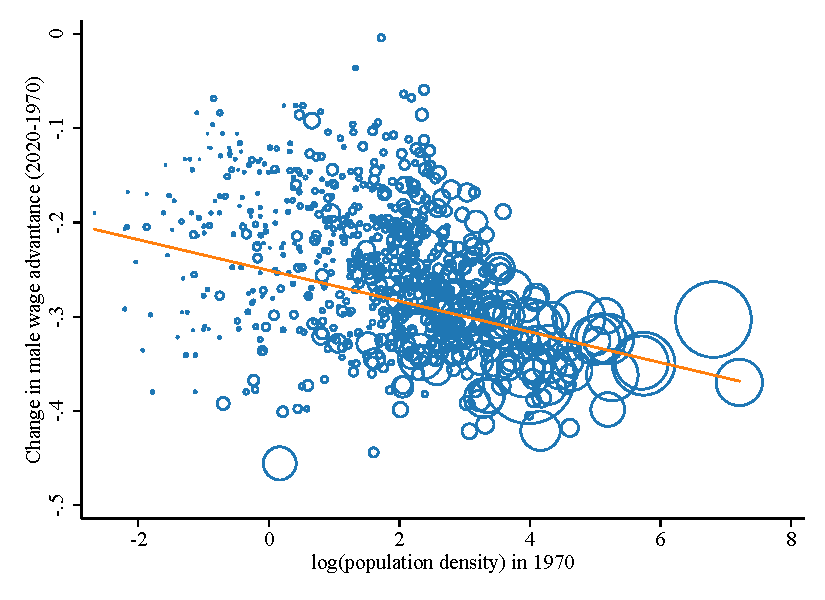
\includegraphics[width=.75\textwidth]{../2_analysis/output/figures/change_in_gap}
\end{figure}

\end{frame}
\begin{frame}{Fact 3: The gender gap - density relation has inverted}  
	\label{slide:baseline}
	\textbf{\alert{Regression specification:}}	$w^{men}_{rt}-w^{women}_{rt}=\alpha_{rt}+\beta_{t}\ln(density)_{rt}$
	\begin{figure}[!h]
\centering
\caption{Coefficient on population density $ \beta_t $}
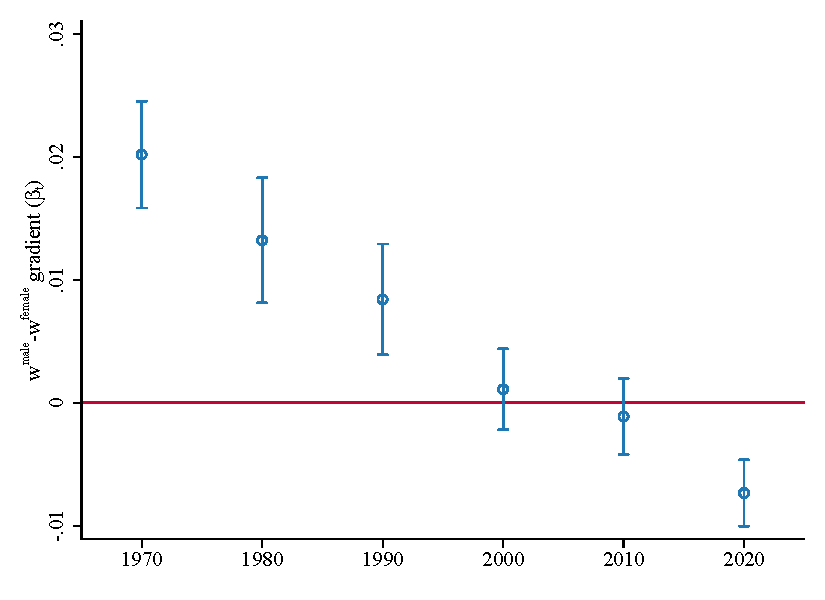
\includegraphics[width=.6\textwidth]{../2_analysis/output/figures/baseline_gradients_l_czone_density_full_time}
\par \begin{minipage}[h]{\textwidth}{\scriptsize\textbf{Note:} figure restricts to CZ with more than 1 people per km$^2$. Bars show 95\% robust confidence intervals.}\end{minipage}
\end{figure}

	\beamerbutton{\hyperlink{slide:distribution}{Distribution illustration}}
\end{frame}
\begin{frame}{How big are these coefficients?}  
		\begin{center}
\begin{threeparttable}[!h]
\caption{Male advantange changes implied by estimated elasticities}
\label{tab:IC}
\begin{tabular}{lcccccc}
\toprule
\toprule
\textbf{}&\multicolumn{1}{c}{\textbf{1970}}&\multicolumn{1}{c}{\textbf{1980}}&\multicolumn{1}{c}{\textbf{1990}}&\multicolumn{1}{c}{\textbf{2000}}&\multicolumn{1}{c}{\textbf{2010}}&\multicolumn{1}{c}{\textbf{2020}} \\
\midrule
Density elasticity $ (\beta ) $&       0.020         &       0.013         &       0.008         &       0.001         &      -0.001         &      -0.007         \\
 \hspace{3mm} s.d. wage gap &       0.073         &       0.077         &       0.060         &       0.049         &       0.049         &       0.050         \\
$ \hspace{3mm}\beta / sd $&       0.278         &       0.173         &       0.141         &       0.022         &      -0.023         &      -0.146         \\
\midrule IC range   &       0.029         &       0.019         &       0.013         &       0.002         &      -0.002         &      -0.012         \\
\hspace{3mm} (\% mean gap) &       0.065         &       0.047         &       0.040         &       0.007         &      -0.009         &      -0.064         \\
 \midrule 90 - 10 pctile range  &       0.061         &       0.040         &       0.027         &       0.004         &      -0.004         &      -0.025         \\
\hspace{3mm} (\% mean gap)&       0.137         &       0.097         &       0.082         &       0.014         &      -0.018         &      -0.133         \\
\bottomrule
\bottomrule
\end{tabular}
\begin{tablenotes}
\item \footnotesize \textit{Note:} changes based on unweighted estimated elasticities. Sample restricted to full-time year-round workers. Table generated on 28 Sep 2020 at 15:15:18.
\end{tablenotes}
\end{threeparttable}
\end{center}

\end{frame}
\begin{frame}{What can account for the change in the density-gradient?}
	\label{slide:controls}
	\textbf{\alert{Regression specification:}} $w^{men}_{rt}-w^{women}_{rt}=\alpha_{rt}+\beta_{t}\ln(density)_t$
	\begin{figure}[!h]
\centering
\caption{Coefficient on population density $ \beta_t $ controlling for worker characteristics}
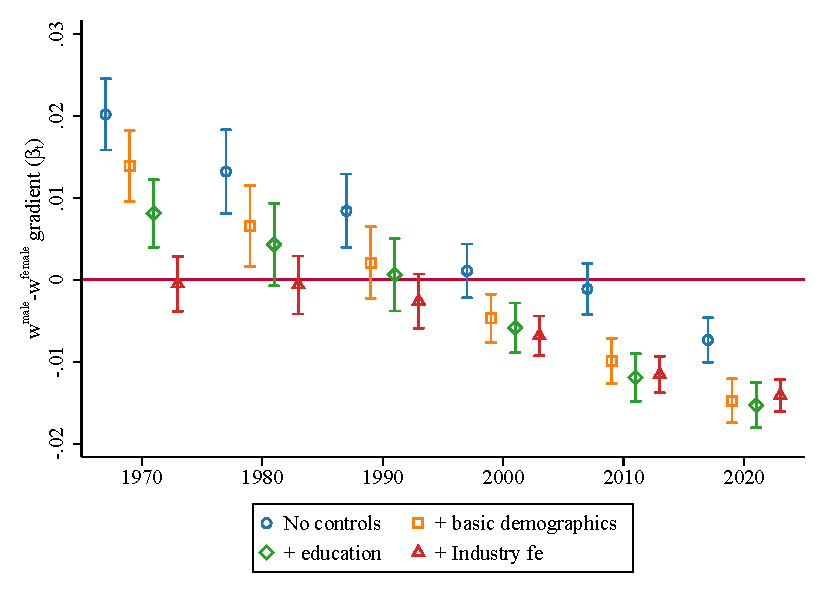
\includegraphics[width=.6\textwidth]{../2_analysis/output/figures/with_control_gradients_individual_l_czone_density_full_time}
\par \begin{minipage}[h]{\textwidth}{\tiny\textbf{Note:} figure restricts to CZ with more than 1 people per km$^2$. The regressions are done on data aggregated at the CZ level after residualizing individual-level characteristics. Bars show 95\% confidence intervals. Errors clustered at the CZ-level.}\end{minipage}
\end{figure}

	\beamerbutton{\hyperlink{slide:residual}{How do I control for individual characteristics?}}
\end{frame}


\appendix

\begin{frame}{The geography of the gender gap in 2020}
\label{slide:map}
\begin{figure}[!h]
\centering
\caption{The gender gap in the US in 2020}
\label{fig:gap_map2020}
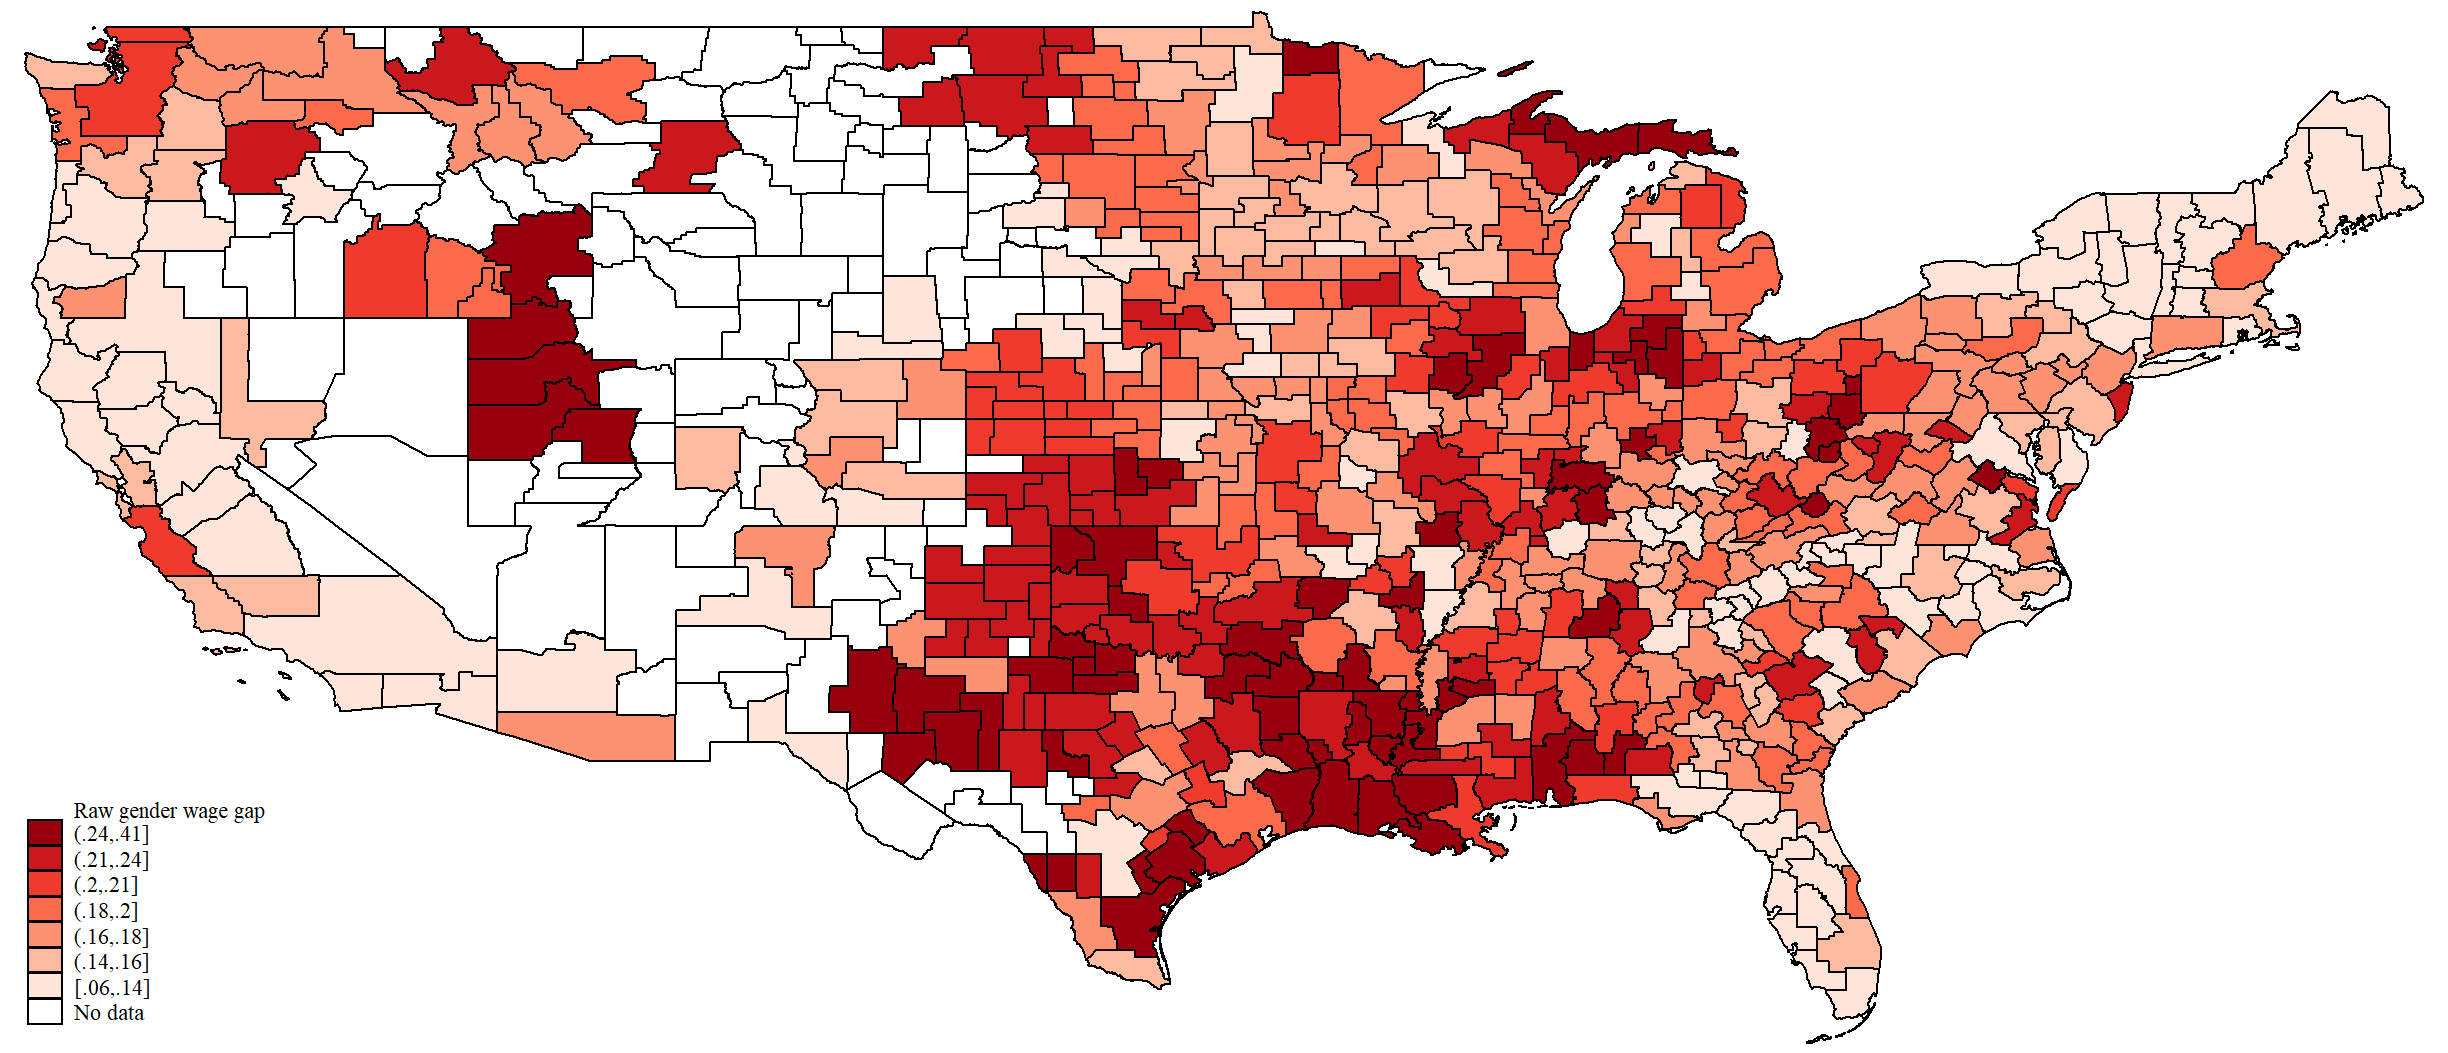
\includegraphics[width=1\textwidth]{../2_analysis/output/figures/raw_wage_map2020_full_time}
\par \begin{minipage}[h]{\textwidth}{\tiny\textbf{Note:} darker colors denote higher relative wages for men. Figure restricts to czones with population densities above 1 person per km$^2$ and full-time year-round workers.}\end{minipage}
\end{figure}

\beamerbutton{\hyperlink{slide:fact1}{Return}}

\end{frame}

\begin{frame}{20-year auto-correlation coefficient is above 50\%} 
	\label{slide:persistence}
	\textbf{\alert{Regression specification:}} $w^{men}_{rt}-w^{women}_{rt}=\alpha_{rt}+\beta_{t}(w^{men}_{rt-j}-w^{women}_{rt-j})$
	\begin{figure}[!h]
\centering
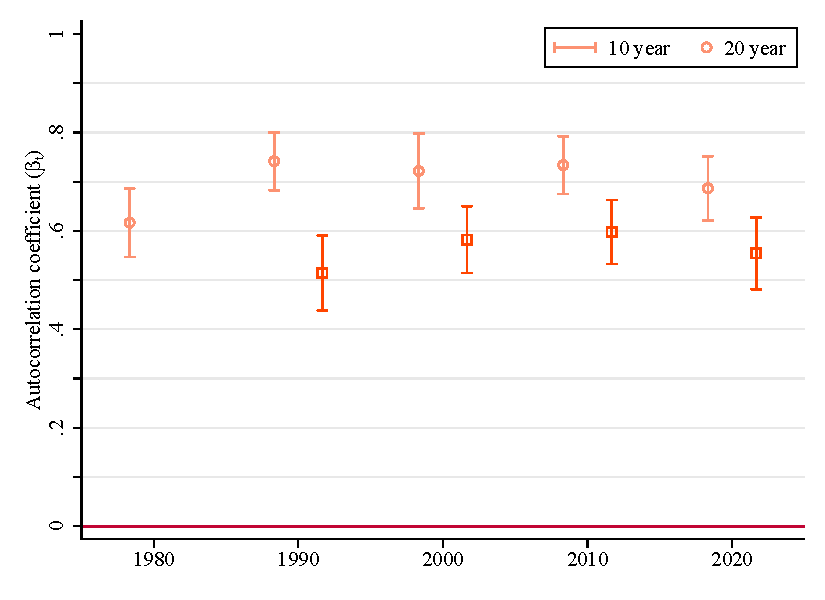
\includegraphics[width=.6\textwidth]{../2_analysis/output/figures/cz_gender_gap_persistence_full_time}
\par \begin{minipage}[h]{\textwidth}{\scriptsize\textbf{Note:} figure restricts to CZ with more than people per km$^2$ and full-time year-round workers.. Bars show 95\% robust confidence intervals. Standard errors are clustered at the CZ level. Dependent and independent variables are standardized}\end{minipage}
\end{figure}

\beamerbutton{\hyperlink{slide:fact1}{Return}}
\end{frame}
\begin{frame}{Residualization procedure}
	\label{slide:residual}
	\begin{enumerate}
		\item Run the regression on \alert{individual} level data:
		\beqns
			wage_{igrt}=X_{igrt}\gamma_t+\lambda_{grt}+\varepsilon_{igrt}
		\eeqns
		where $i,g,r,t$ index individual, sex, CZ and decade respectively. I impose the \alert{same} return on individual level characteristics across sex and CZ.
		\item Run the following regression at the CZ level:
		\beqns
			\lambda_{mrt}-\lambda_{frt}=\alpha_t+\beta_{t}\ln(density)_{rt}
		\eeqns
		no weight is imposed on the CZ-level regressions \citep{Solon2015a}.
		\beamerbutton{\hyperlink{slide:controls}{Return}}
	\end{enumerate}
\end{frame}

\begin{frame}{Low vs high density CZ}
	\label{slide:distribution}
	\begin{figure}[!h]
\centering
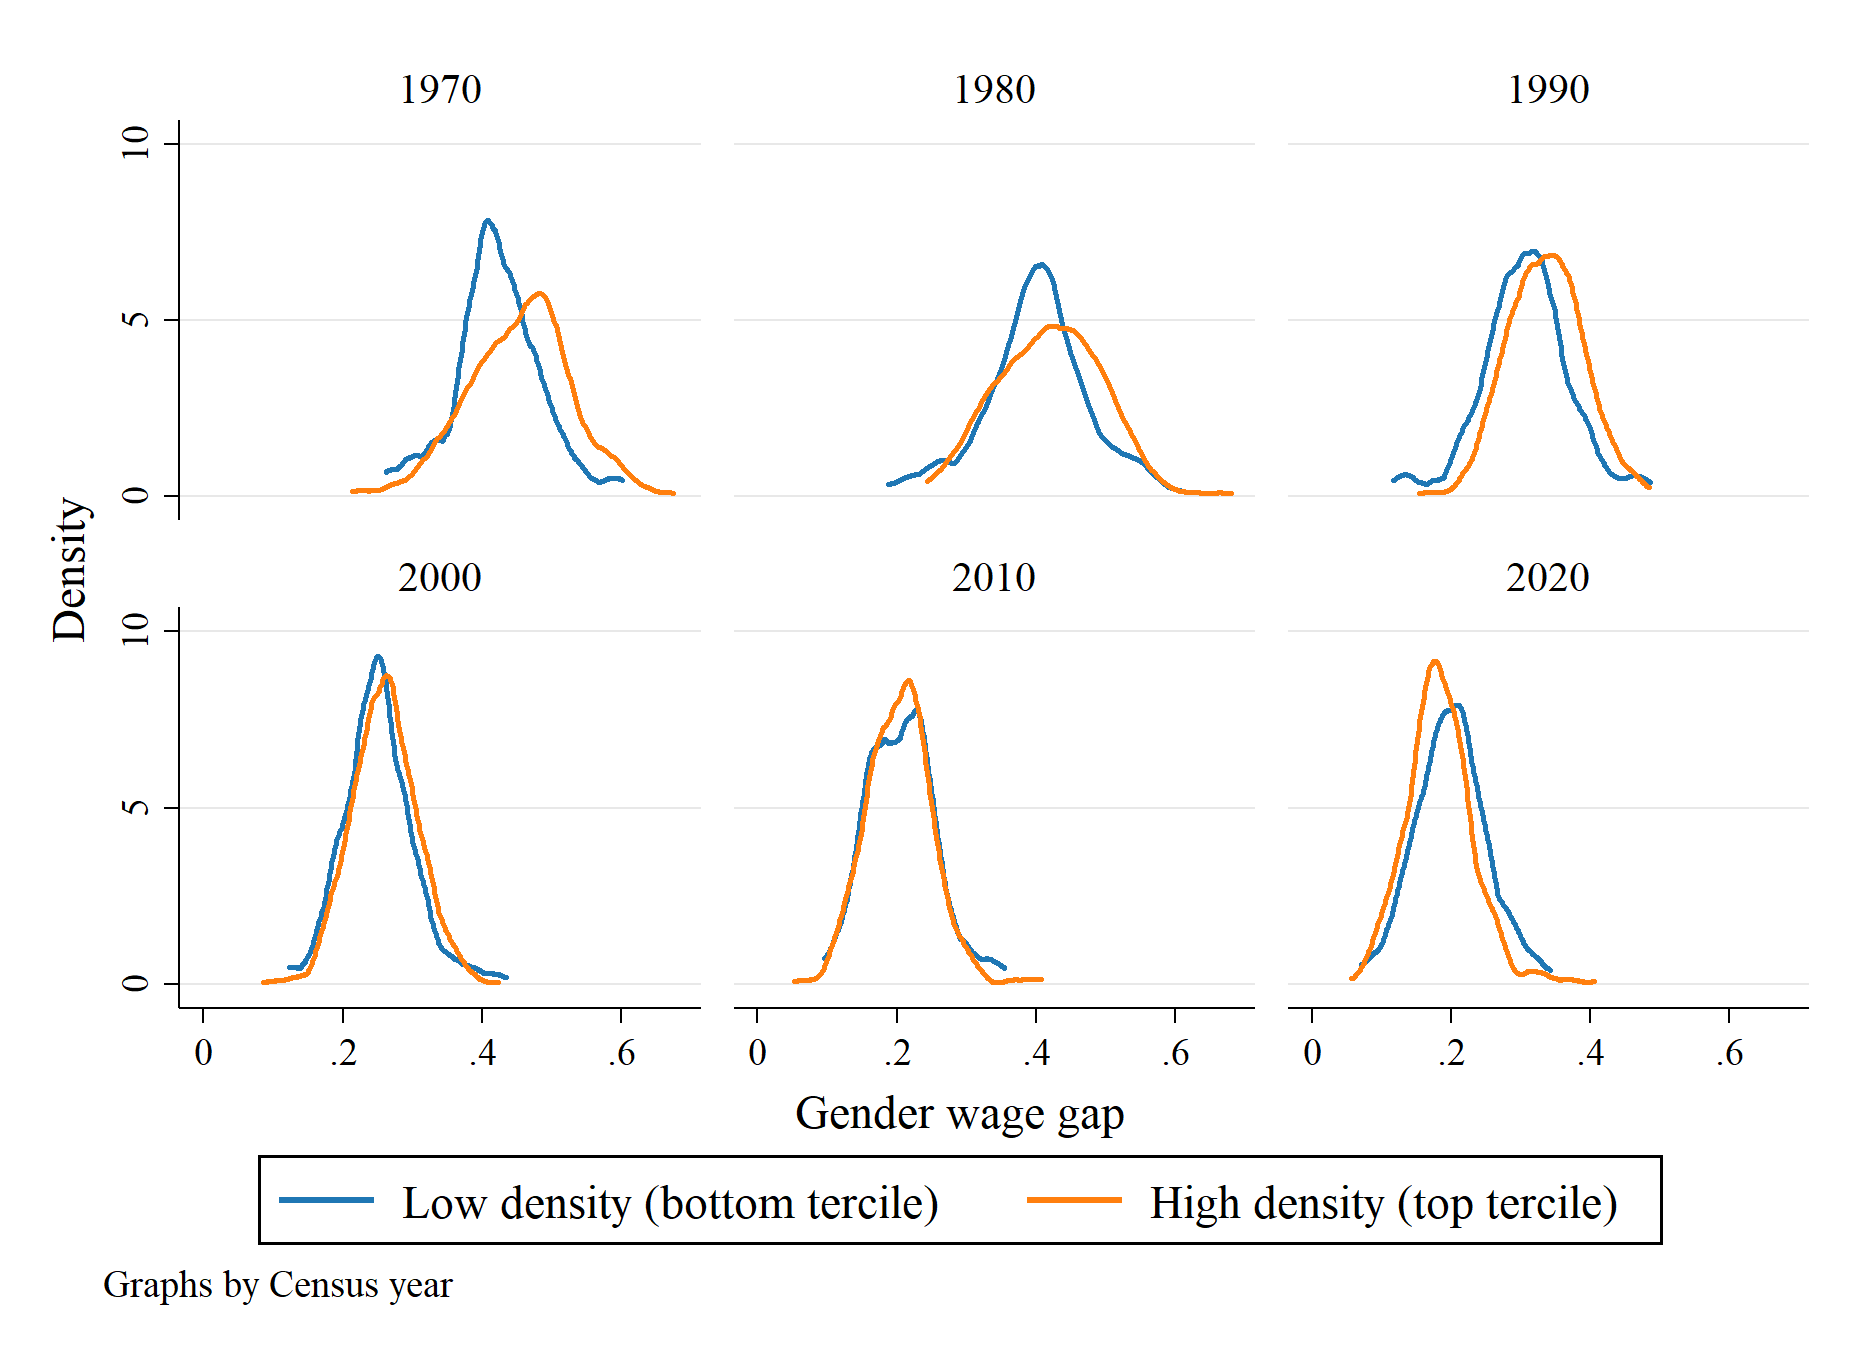
\includegraphics[width=.8\textwidth]{../2_analysis/output/figures/distribution_gap_movement_full_time}
\par \begin{minipage}[h]{\textwidth}{\scriptsize\textbf{Note:} figure restricts to CZ with more than 1 people per km$^2$. Figure generated on 28 Sep 2020 at 15:56:45. Figure generated using the dofile code\_files/kernel\_density\_movement.do.}\end{minipage}
\end{figure}

	\beamerbutton{\hyperlink{slide:baseline}{Return}}
\end{frame}


\begin{frame}{Within-marital status graphs}
	\label{slide:married}
	\textbf{\alert{Regression specification:}}	$w^{men}_{rt}-w^{women}_{rt}=\alpha_{rt}+\beta_{t}\ln(density)_{rt}+ \dots$
	\begin{figure}[!h]
\centering
\caption{Coefficient on population density $ \beta_t $ controlling for worker characteristics}
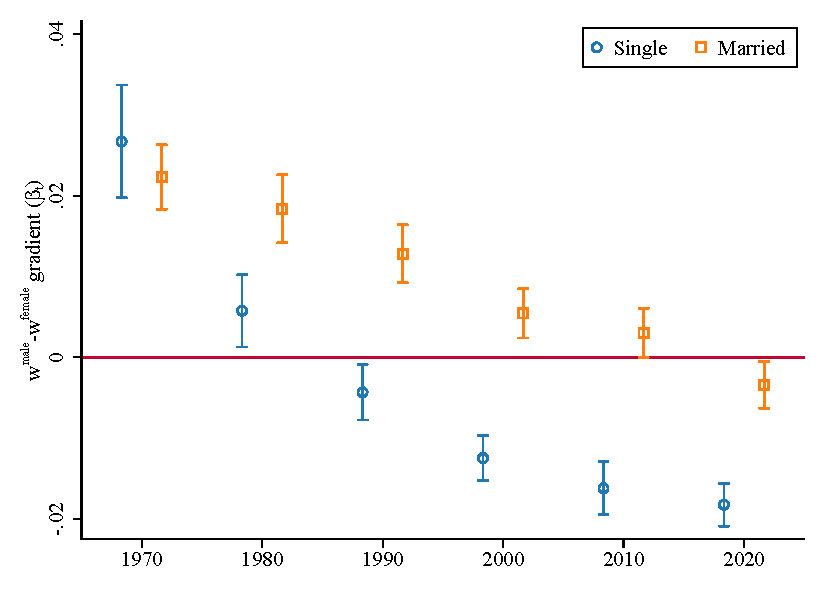
\includegraphics[width=.6\textwidth]{../2_analysis/output/figures/by_married_czone_l_czone_pop_full_time}
\par \begin{minipage}[h]{\textwidth}{\tiny\textbf{Note:} figure restricts to CZ with more than 1 people per km$^2$. Regression includes census division. The regressions are done on data aggregated at the CZ level. Bars show 95\% robust confidence intervals. Standard errors clustered at the CZ level. Figure generated on 20 Oct 2020 at 09:16:34. Figure generated using the dofile 2\_analysis/code\_files/write\_regression\_coefplots.do.}\end{minipage}
\end{figure}

	\beamerbutton{\hyperlink{slide:baseline}{Return}}
\end{frame}

\begin{frame}{Within-having children status graphs}
	\label{slide:has_children}
	\textbf{\alert{Regression specification:}}	$w^{men}_{rt}-w^{women}_{rt}=\alpha_{rt}+\beta_{t}\ln(density)_{rt}+ \dots$
	\begin{figure}[!h]
\centering
\caption{Coefficient on population density $ \beta_t $ conditional conditional on having children}
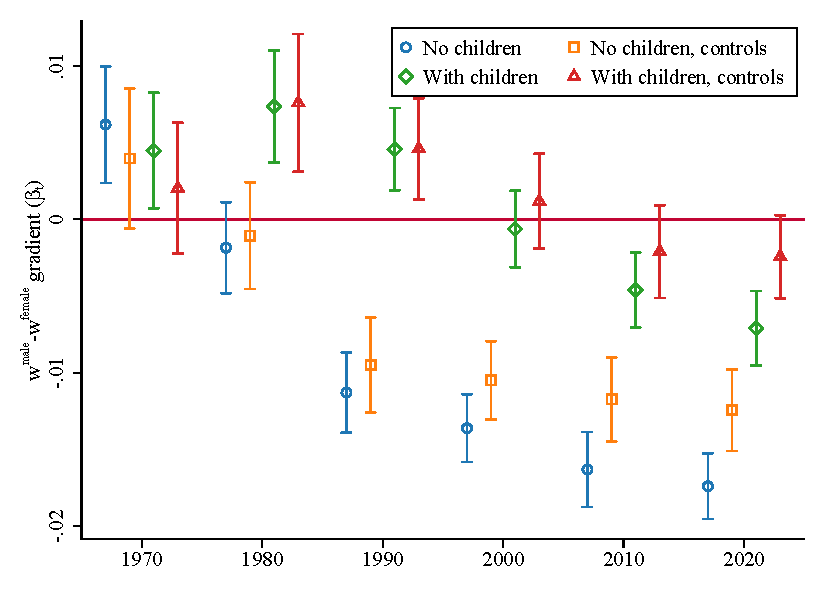
\includegraphics[width=.6\textwidth]{../2_analysis/output/figures/by_children_l_czone_pop_full_time}
\par \begin{minipage}[h]{\textwidth}{\tiny\textbf{Note:} figure restricts to CZ with more than 1 people per km$^2$. Regression includes census division fixed-effects. The regressions are done on data aggregated at the CZ level. Bars show 95\% robust confidence intervals. Standard errors clustered at the CZ level. Figure generated on 20 Oct 2020 at 09:56:35. Figure generated using the dofile 2\_analysis/code\_files/write\_regression\_coefplots.do.}\end{minipage}
\end{figure}

	\beamerbutton{\hyperlink{slide:baseline}{Return}}
\end{frame}


\begin{frame}{Is this about gender? pattern doesn't appear for across race}
	\label{slide:race}
	\textbf{\alert{Regression specification:}}	$w^{white}_{rt}-w^{black}_{rt}=\alpha_{rt}+\beta_{t}\ln(density)_{rt}+ \dots$
	\begin{figure}[!h]
\centering
\caption{Coefficient on population density $ \beta_t $}
\label{fig:race_gradient}
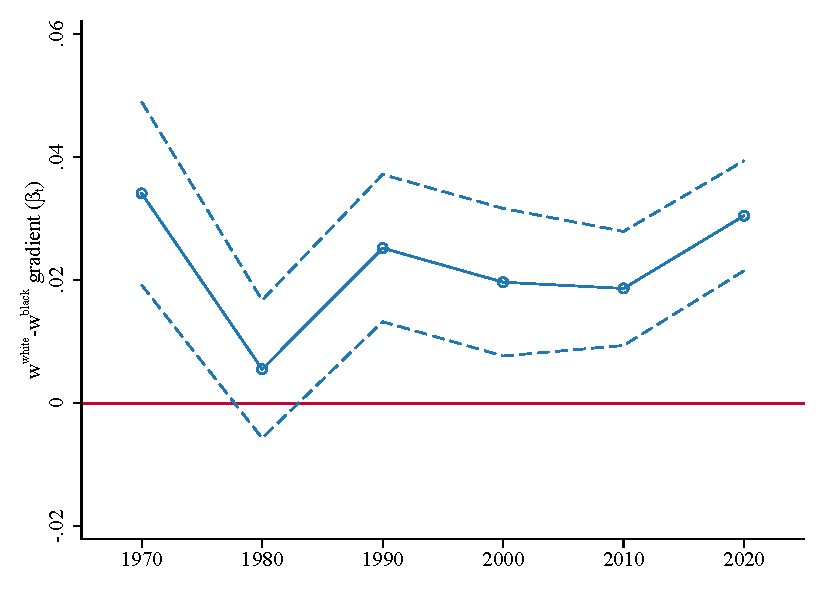
\includegraphics[width=.6\textwidth]{../2_analysis/output/figures/baseline_race_gradients_l_czone_density_full_time}
\par \begin{minipage}[h]{\textwidth}{\tiny\textbf{Note:} figure restricts to CZ with more than 1 people per km$^2$. Bars show 90\% confidence intervals. Standard errors clustered at the CZ level. The figure restricts to year-round full time men workers. Figure generated on 30 Nov 2020 at 11:17:27. Figure generated using the dofile 2\_analysis/code\_files/write\_regression\_coefplots.do.}\end{minipage}
\end{figure}

	\beamerbutton{\hyperlink{slide:baseline}{Return}}		
\end{frame}

%\begin{frame}{Motivation}
%\begin{figure}
%	\includegraphics[width=\textheight]{../2_analysis/output/figures/article.png}
%\end{figure}
%\end{frame}
%\begin{frame}{Motivation}
%\bitem
%	\item People living in denser labor markets are paid higher wages giving rise to an \alert{\textbf{urban wage premium}} \citep{Glaeser2001,Moretti2011}. Much less attention has been paid to the variation of this premium differs across \textbf{\alert{gender}} \citep{Bacolod2017,Phimister2005,Beaudry2014}.
%	\item Here I document three facts about wages, the gender wage gap, and population density across commuting zones (CZ) in the US.
%	\benu
%		\item The wage-population density gradient differs across genders.
%		\item While today, women's wages increase more with population density than men's, in 1970 the opposite was true.
%		\item The relationship between the gender gap and population density has inverted between 1970-2020.
%	\eenu 
%\eitem 
%\end{frame}

%\begin{frame}{Literature}
%	\bitem
%	\item 
%	\eitem 
%\end{frame}
%\begin{frame}{Data}
%	\bitem
%	\item \textbf{\alert{Data:}} IPUMS decennial census samples from 1950 to 2000 and 5-year 2011 and 2018 ACS.
%	\item \textbf{\alert{Sample:}} all people aged 18-65, not living in group quarters.
%	\item \textbf{\alert{Definition of labor market:}} \cite{Autor2013} CZ delineation. I focus on the 722 CZ in mainland US.
%	\item For most graphs I restrict to CZ with population densities in 1950 of at least 1 person per square km.
%	\item \alert{\textbf{Variables of interest}} are $w^{male}, w^{female},$ and $w^{male}-w^{female}$, where $w$ is the log of average hourly wage in the the CZ.
%	\eitem 
%\end{frame}
%
%\begin{frame}{Basic facts}
%	\begin{enumerate}
%		\item There is substantial dispersion in the unadjusted gender-wage gap across CZ in the US.
%		\item This dispersion in the gap has persisted over 1970-2020 $\implies$ s.d. $\approx$ \textbf{\alert{20\%}} of the mean gap.
%		\item CZ-level gender gaps are \textbf{\alert{persistent}}.
% 	\end{enumerate}
% 	Question: what explains these differences? Should we care about them.	
%\end{frame}



%\begin{frame}{Dispersion in the gap has remained over the whole period} 
%	\begin{figure}[!h]
\centering
\caption{Evolution of raw gender gap across CZ}
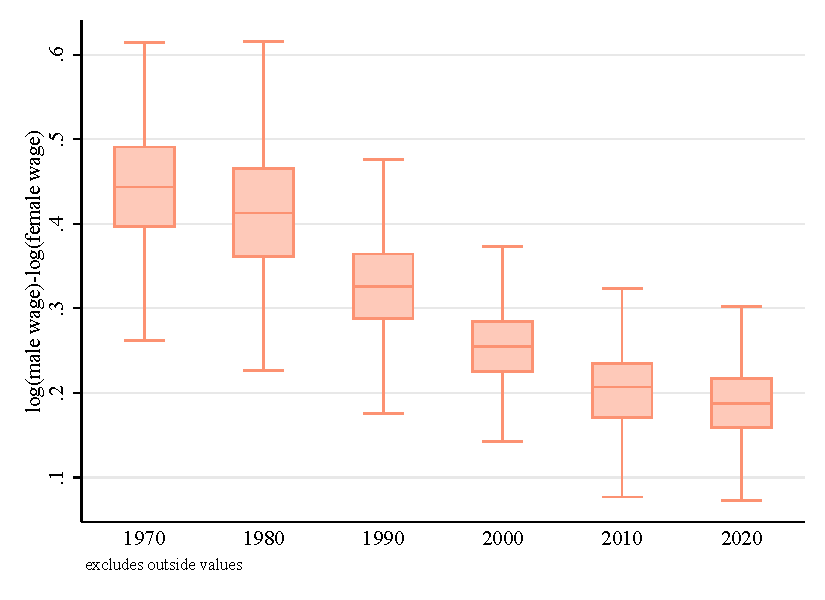
\includegraphics[width=.6\textwidth]{../2_analysis/output/figures/cz_gap_dispersion_full_time}
\par \begin{minipage}[h]{\textwidth}{\scriptsize\textbf{Note:} figure restricts to CZ with more than people per km$^2$ and full-time year-round workers..}\end{minipage}
\end{figure}

%\end{frame}

%\begin{frame}{Across CZ differences in the gap are persistent} 
%	I run the regression,
%	\beqns
%			w^{male}_{rt}-w^{female}_{rt}=\alpha_t+\beta_t(w^{male}_{r1970}-w^{female}_{r1970})
%	\eeqns
%	\begin{figure}[!h]
\centering
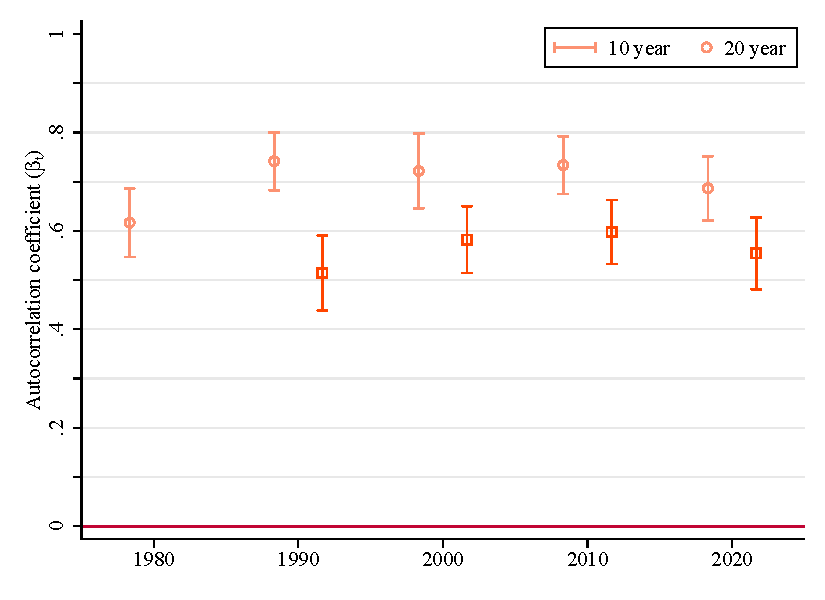
\includegraphics[width=.6\textwidth]{../2_analysis/output/figures/cz_gender_gap_persistence_full_time}
\par \begin{minipage}[h]{\textwidth}{\scriptsize\textbf{Note:} figure restricts to CZ with more than people per km$^2$ and full-time year-round workers.. Bars show 95\% robust confidence intervals. Standard errors are clustered at the CZ level. Dependent and independent variables are standardized}\end{minipage}
\end{figure}

%\end{frame}


%\section{Basic regressions}
%
\begin{frame}{Accounting for individual characteristics}
\alert{\textbf{Route A}}: \newline
\begin{enumerate}
	\item Run on individual-level data:
	\beqns
		wage_{irt}^g=X_{iry}^g\gamma_t+\lambda_{rt}^g+\varepsilon_{irt}^g
	\eeqns
	\item In a second stage run:
	\beqns
		\hat{\lambda}_{rt}^{male}-\hat{\lambda}_{rt}^{female}=\tau_t+\beta_t\log(density)_{rt}+\varepsilon_{irt}^g
	\eeqns
\end{enumerate}
\end{frame}
\begin{frame}{Accounting for individual characteristics}
\alert{\textbf{Route B}}: \newline
If wages are determined at the individual level by the model:
\beqns
	w_{irt}^g=X_{irt}^g\gamma_t+\tau_tmale_i+\varepsilon_t
\eeqns
By aggregating at the CZ level this model becomes:
\beqns
w^{male}_{rt}-w^{female}_{rt}=\tau_t+ (\bar{X}_{rt}^{male}-\bar{X}_{rt}^{female})\gamma_t+u_t
\eeqns
Thus I run regressions of the form:
\beqns
w^{male}_{rt}-w^{female}_{rt}=\tau_t+ (\bar{X}_{rt}^{male}-\bar{X}_{rt}^{female})\gamma_t+\beta_t\log(density)_{rt}+u_t
\eeqns
\end{frame}
\begin{frame}{Route A}
\begin{figure}[!h]
\centering
\caption{Coefficient on population density $ \beta_t $ controlling for worker characteristics}
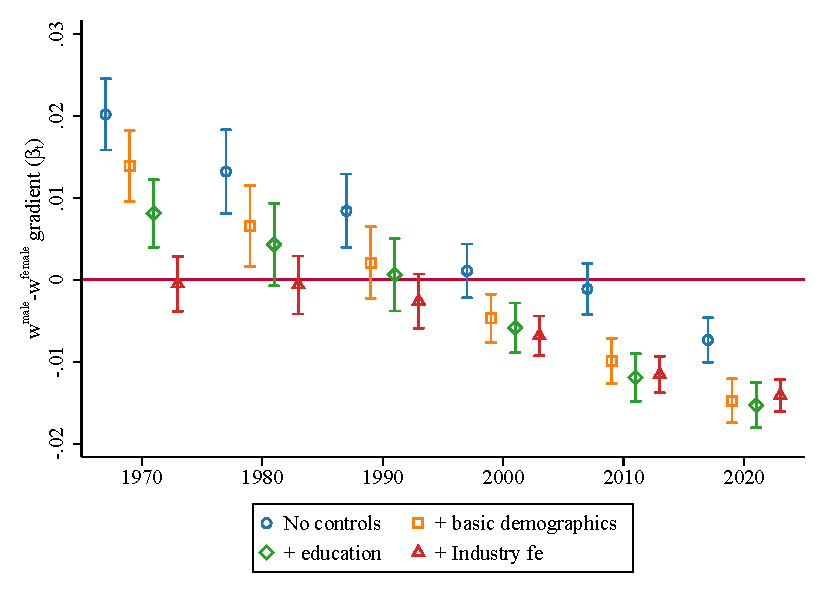
\includegraphics[width=.6\textwidth]{../2_analysis/output/figures/with_control_gradients_individual_l_czone_density_full_time}
\par \begin{minipage}[h]{\textwidth}{\tiny\textbf{Note:} figure restricts to CZ with more than 1 people per km$^2$. The regressions are done on data aggregated at the CZ level after residualizing individual-level characteristics. Bars show 95\% confidence intervals. Errors clustered at the CZ-level.}\end{minipage}
\end{figure}

\end{frame}
\begin{frame}{Route B}
\begin{figure}[!h]
\centering
\caption{Coefficient on population density $ \beta_t $ controlling for worker characteristics}
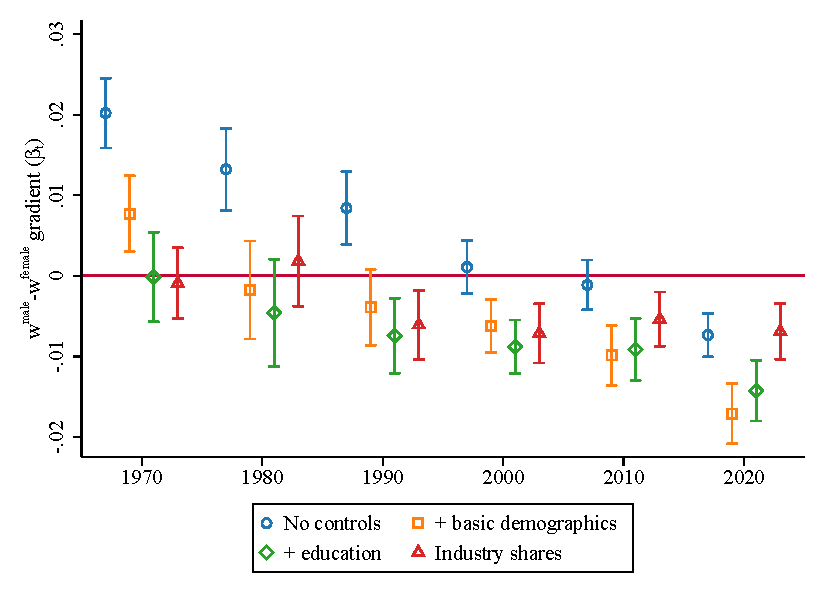
\includegraphics[width=.6\textwidth]{../2_analysis/output/figures/with_control_gradients_l_czone_density_full_time}
\par \begin{minipage}[h]{\textwidth}{\scriptsize\textbf{Note:} figure restricts to CZ with more than 1 people per km$^2$. The regressions are done on data aggregated at the CZ level. Bars show 95\% robust confidence intervals.}\end{minipage}
\end{figure}

\end{frame}


\bibliographystyle{apalike}
\bibliography{../../../../CentralLibrary/Papers/library}{}
\end{document}

